\documentclass{article}
\usepackage{mathtools}
\usepackage{amsfonts}
\usepackage{amssymb}
\usepackage{fullpage}
\usepackage{amsmath}
\usepackage{multirow}
\usepackage{graphicx}
\usepackage{caption}
\usepackage{subcaption}
\usepackage{float}
\usepackage{hyperref}
\usepackage{graphicx}
\usepackage{caption}
\usepackage{subcaption}
\usepackage[utf8]{inputenc}
\usepackage{tikz}
\usetikzlibrary{shapes.geometric, arrows}

\tikzstyle{startstop} = [rectangle, rounded corners, minimum width=3cm, minimum height=1cm,text centered, draw=black, fill=red!30]
\tikzstyle{randomAlaska} = [trapezium, trapezium left angle=80, trapezium right angle=100, minimum width = 1cm, minimum height=1cm, text centered, draw=black, text width = 3cm, node distance=3cm, fill=blue!30]
\tikzstyle{randomArabia} = [trapezium, trapezium left angle=80, trapezium right angle=100, minimum width = 1cm, minimum height=1cm, text centered, draw=black, text width = 3cm, node distance=3cm, fill=red!80]
\tikzstyle{randomCaribbean} = [trapezium, trapezium left angle=80, trapezium right angle=100, minimum width = 1cm, minimum height=1cm, text centered, draw=black, text width = 3cm, node distance=3cm, fill=black!20]
\tikzstyle{process} = [rectangle, minimum width=3cm, minimum height=1cm, text centered, text width=3cm, draw=black, fill=orange]
\tikzstyle{fixedEffects} = [diamond, minimum width=3cm, minimum height=1cm, text centered, draw=black, node distance=3cm, fill=green!30]
\tikzstyle{arrow} = [thick,->,>=stealth]
\author{Dillon Flannery}
\title{Hierarchical Model For Holland America Cruises}


\begin{document}

	\maketitle
		\tableofcontents
		\newpage
	\section{Introduction} So far I have tried to fit a variety of different models to the data from Holland America which includes passenger information for about 1.8 million passengers that came on Holland Cruises for the last 3 years. An general linear regression was found to fit the data reasonably well. Using a Bayesian linear regression did not improve the fit of the model significantly to warrant the extensive procedure necessary for specifying prior distributions. However, Bayesian techniques are not without merit as the following results show. Using hierarchical models produced demonstrably better fit measured by root mean squared error. These types of models work by breaking the sample into a set of groups. There are what is termed `fixed effects' and `random effects' for each of the groups. The fixed effects are shared across groups and the parameter esitmates are the same, hence the name, they are `fixed' for the entire model. There are also random parameters. These are specific to each group. They are estimated using the data only for one group, so they should theoretically fit the data better. The graphic below is trying to get at this idea. The horizontal lines between the fixed effects is showing that those are shared between models. The entire dataset is used to generate those effects. The curved lines connecting each trade to a random effect is attempting to show that each trade has its own cruiselength parameter. \\
	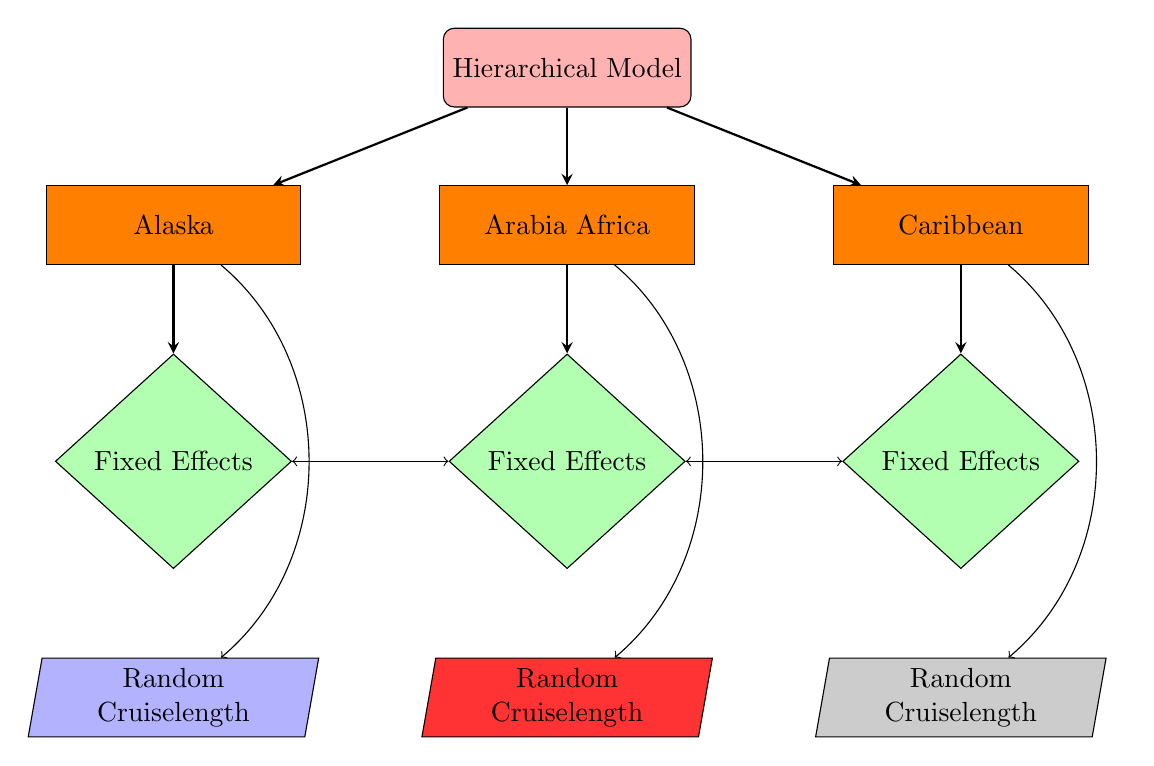
\begin{tikzpicture}[node distance=2cm][line/.style={<->,shorten >=0.4cm,shorten <=0.4cm},thick]
	
	\node (model) [startstop] {Hierarchical Model};
	
	\node (arabia) [process, below of=model] {Arabia Africa};
	\node (alaska) [process, left of=arabia, node distance = 5cm] {Alaska};
	\node (caribbean) [process, right of=arabia, node distance = 5cm] {Caribbean};
	\node (fixedAlaska) [fixedEffects, below of=alaska] {Fixed Effects};
	\node (fixedArabia) [fixedEffects, below of=arabia] {Fixed Effects};
	\node (fixedCaribbean) [fixedEffects, below of=caribbean] {Fixed Effects};
	\node (randomAlas) [randomAlaska, below of=fixedAlaska] {Random Cruiselength};
	\node (randomArab) [randomArabia, below of=fixedArabia] {Random Cruiselength};
	\node (randomCar) [randomCaribbean, below of=fixedCaribbean] {Random Cruiselength};
	
	\draw [arrow] (model) -- (arabia);
	\draw [arrow] (model) -- (alaska);
	\draw [arrow] (model) -- (caribbean);
	\draw [arrow] (arabia) -- (fixedArabia);
	\draw [arrow] (alaska) -- (fixedAlaska);
	\draw [arrow] (caribbean) -- (fixedCaribbean);
	\path [->] (alaska) edge [bend left=50]  (randomAlas);
	\path [->] (arabia) edge [bend left=50]  (randomArab);
	\path [->] (caribbean) edge [bend left=50]  (randomCar);
	\path [<->] (fixedAlaska) edge (fixedArabia) ;
	\path [<->] (fixedArabia) edge (fixedCaribbean);
	\end{tikzpicture}\\
	
	\section{Model} The model I chose to estimate for the data is the following, 
	\[
	Y = \beta_{0i} + \beta_{1}\text{NTR P.C.D.}\footnote{Book to cruise day} + \beta_2 \text{AGE} + \beta_3 \text{B.C.T.D.} + \beta_{4i} \text{CRUISELENGTH} + \beta_{5}\text{SHIPNAME} + \beta_6 \text{NATION} + \beta_7 
	\]
	\[
	\text{ROOM} + \beta_8 \text{LOYALTY} + \beta_9 \text{GENDER} + \text{RANDOM ERROR} 
	\]
	
	\[ 
	\beta_{0i} \sim N(\gamma_0 + \gamma_1 x_i,\sigma^2_i), \  \beta_{4i} \sim N(\phi_0 + \phi_1 z_i, \epsilon^2_i), i = 1, 2...14 \footnote{Each random component (intercept and cruise length here) has an overall group mean and a component specific to its trade. Each random component in effect has its own regression with error term labelled above as $ \sigma $ and $ \epsilon $. The interpretation of $ x_i $ is daily revenue for trade $ i $, and similarly $ z_i $  is the cruise length for trade $ i $. }
	\]
	
	For each trade we will have a random intercept. This is comparable to a dummy variable for trade in normal linear regression. What is novel in the Bayesian hierarchical approach is the ability to predict a random slope intercept for cruise length This should allow us to fit the data better since the cruise length is tailored to that specific trade. \\
	
	Note, the output from these models is verbose! When one of these models is run a separate regression is made for each of the 14 trades in our dataset. Then there are 8 different departments. For each of the departments there are 34 fixed effects and 28 random effects, totalling 62 different parameters for each model so multiplied by 8 that makes 496 different parameter estimates So to be complete I have included everything that is possible, the full model for each of the 8 departments but it is a lot of information. The estimations are also costly in terms of computing power. To run all the models once took over 8 hours on my machine. \\
	
	\section{Results} Below is a result of the model fit. For our dataset 80\% of the dataset was used to get parameter estimates, the other 20\% for validation. The measure of goodness-of-fit used was mean squared error and root mean squared error. This is calculated by taking the actual and subtracting the predicted value, squaring it so under predictions are also penalized, then summing the total. The square root is taken to represent a quasi-standard deviation of the error. In the table below these are shown, MSE stands for `mean-squared error' and H-model stands for hierarchical model. The L-model is the regular linear regression model, and the `Root MSE' is the square root of the MSE. The difference is also taken between the hierarchical and the linear model. Negative values would indicate that the root MSE of the hierarchical model was smaller, and therefore a better fit (its predictions were closer to the actuals). For each department these statistics were calculated and tabulated below. 
	
	
			
	\begin{table}[H]
		\centering
		\scalebox{.8}{
			\begin{tabular}{rrrrrr}

				TRADE & MSE  H-Model  & MSE L-Model & Root  MSE  H-Model & Root  MSE L-Model & Difference  (H  -  L) \\
								\hline 
								\hline 
				ALASKA & 146480723.715 & 146505542.697 & 12102.922 & 12103.947 & -1.025 \\
				ARABIA  AFRICA & 123256.596 & 122784.406 & 351.079 & 350.406 & 0.673 \\
				ASIA  ORIENT & 13866142.98 & 13885447.583 & 3723.727 & 3726.318 & -2.591 \\
				BERMUDA & 910551.859 & 911229.909 & 954.228 & 954.584 & -0.355 \\
				CANADA  NEW  ENGLAND & 12490797.39 & 12500664.972 & 3534.232 & 3535.628 & -1.396 \\
				CARIBBEAN & 25701027.171 & 25811422.492 & 5069.618 & 5080.494 & -10.876 \\
				COASTAL & 189255.249 & 195217.738 & 435.035 & 441.835 & -6.8 \\
				EUROPE & 68221462.98 & 68412286.072 & 8259.629 & 8271.172 & -11.543 \\
				HAWAII & 1233072.92 & 1238557.265 & 1110.438 & 1112.905 & -2.467 \\
				MEXICO & 966816.777 & 967405.664 & 983.268 & 983.568 & -0.299 \\
				PANAMA  CANAL & 1907050.152 & 1916299.542 & 1380.96 & 1384.305 & -3.345 \\
				SOUTH  AMERICA & 10714887.734 & 10767709.157 & 3273.36 & 3281.419 & -8.058 \\
				SOUTH  PACIFIC & 12098975.543 & 12175701.3 & 3478.358 & 3489.37 & -11.012 \\
				WORLD  VOYAGE & 1290986.993 & 1408878.038 & 1136.216 & 1186.962 & -50.746 \\
				\hline
				\hline 
			\end{tabular}
		}
		\caption{Shorex estimations}
	\end{table}
	
\begin{table}[H]
	\centering
	\scalebox{.8}{
	\begin{tabular}{rrrrrr}
		TRADE & MSE  H-Model & MSE L-Model & Root MSE H-Model & Root MSE L-Model & Difference (H - L) \\
		\hline 
		\hline 
		ALASKA & 262623062.281 & 262623973.883 & 16205.649 & 16205.677 & -0.028 \\
		ARABIA AFRICA & 4672.251 & 4682.04 & 68.354 & 68.425 & -0.072 \\
		ASIA ORIENT & 10321170.363 & 10326980.769 & 3212.658 & 3213.562 & -0.904 \\
		BERMUDA & 7103609.713 & 7104066.687 & 2665.26 & 2665.346 & -0.086 \\
		CANADA N.E. & 31504693.65 & 31505735.507 & 5612.904 & 5612.997 & -0.093 \\
		CARIBBEAN & 126320125.114 & 126323576.699 & 11239.223 & 11239.376 & -0.154 \\
		COASTAL & 5003924.131 & 5028522.272 & 2236.945 & 2242.437 & -5.491 \\
		EUROPE & 141897357.176 & 141899187.712 & 11912.068 & 11912.145 & -0.077 \\
		HAWAII & 3237384.757 & 3237544.666 & 1799.273 & 1799.318 & -0.044 \\
		MEXICO & 16498787.688 & 16498536.955 & 4061.87 & 4061.839 & 0.031 \\
		PANAMA CANAL & 4734079.304 & 4735122.654 & 2175.794 & 2176.034 & -0.24 \\
		SOUTH AMERICA & 23744849.203 & 23752981.419 & 4872.869 & 4873.703 & -0.834 \\
		SOUTH PACIFIC & 36960400.998 & 36990821.225 & 6079.507 & 6082.008 & -2.501 \\
		WORLD VOYAGE & 1115008.804 & 1123363.329 & 1055.94 & 1059.888 & -3.949 \\
		\hline 
		\hline 
	\end{tabular}
	}
	\caption{Retail estimations}
\end{table}

	\begin{table}[H]
		\centering
		\scalebox{.8}{
\begin{tabular}{rrrrrr}
	TRADE & MSE H-Model & MSE L-Model & Root MSE H-Model & Root MSE -Model & Difference (H - L) \\
	\hline 
	\hline 
	ALASKA & 39776356.339 & 39771545.37 & 6306.85 & 6306.469 & 0.381 \\
	ARABIA AFRICA & 15001.574 & 15079.954 & 122.481 & 122.8 & -0.32 \\
	ASIA ORIENT & 1911799.143 & 1920337.17 & 1382.678 & 1385.762 & -3.084 \\
	BERMUDA & 609549.859 & 609552.545 & 780.737 & 780.738 & -0.002 \\
	CANADA N.E. & 3872751.55 & 3873709.73 & 1967.931 & 1968.174 & -0.243 \\
	CARIBBEAN & 23048651.907 & 23056581.128 & 4800.901 & 4801.727 & -0.826 \\
	COASTAL & 584269.77 & 645273.642 & 764.375 & 803.289 & -38.914 \\
	EUROPE & 16793292.503 & 16800296.89 & 4097.962 & 4098.817 & -0.855 \\
	HAWAII & 565868.52 & 569988.729 & 752.242 & 754.976 & -2.734 \\
	MEXICO & 987300.312 & 988226.654 & 993.63 & 994.096 & -0.466 \\
	PANAMA CANAL & 1161746.767 & 1163183.133 & 1077.844 & 1078.51 & -0.666 \\
	SOUTH AMERICA & 1434889.843 & 1434910.657 & 1197.869 & 1197.878 & -0.009 \\
	SOUTH PACIFIC & 2878582.92 & 2880221.695 & 1696.639 & 1697.122 & -0.483 \\
	WORLD VOYAGE & 119619.501 & 132338.002 & 345.861 & 363.783 & -17.922 \\
	\hline 
	\hline 
\end{tabular}
		}
		\caption{Bar estimations}
	\end{table}
	
	\begin{table}[H]
		\scalebox{.8}{
\begin{tabular}{rrrrrr}
	TRADE & MSE H-Model & MSE L-Model & Root MSE H-Model & Root MSE L-Model & Difference (H - L) \\
	\hline 
	\hline 
	ALASKA & 29367145.722 & 29369034.305 & 5419.146 & 5419.32 & -0.174 \\
	ARABIA AFRICA & 577.015 & 579.498 & 24.021 & 24.073 & -0.052 \\
	ASIA ORIENT & 387935.542 & 388133.181 & 622.845 & 623.003 & -0.159 \\
	BERMUDA & 220804.13 & 220804.174 & 469.898 & 469.898 & 0 \\
	CANADA N.E. & 2213951.281 & 2214276.777 & 1487.935 & 1488.045 & -0.109 \\
	CARIBBEAN & 15129241.553 & 15130222.811 & 3889.633 & 3889.759 & -0.126 \\
	COASTAL & 200623.503 & 201899.169 & 447.91 & 449.332 & -1.422 \\
	EUROPE & 4811353.604 & 4811251.719 & 2193.48 & 2193.457 & 0.023 \\
	HAWAII & 126446.403 & 126655.044 & 355.593 & 355.886 & -0.293 \\
	MEXICO & 1089193.045 & 1089264.671 & 1043.644 & 1043.678 & -0.034 \\
	PANAMA CANAL & 471929.497 & 472291.134 & 686.971 & 687.234 & -0.263 \\
	SOUTH AMERICA & 258763.189 & 258866.499 & 508.688 & 508.789 & -0.102 \\
	SOUTH PACIFIC & 1003496.99 & 1003560.033 & 1001.747 & 1001.778 & -0.031 \\
	WORLD VOYAGE & 10454.025 & 10838.215 & 102.245 & 104.107 & -1.862 \\
	\hline 
	\hline 
\end{tabular}
		}
		\caption{Photo estimations}
	\end{table} 
	
\begin{table}[H]
	\centering 
			\scalebox{.8}{
	\begin{tabular}{rrrrrr}
		TRADE & MSE H-Model & MSE L-Model & Root MSE H-Model & Root MSE L-Model & Difference (H - L) \\
		\hline 
		\hline 
		ALASKA & 45675454.475 & 45677722.674 & 6758.362 & 6758.53 & -0.168 \\
		ARABIA AFRICA & 3635.325 & 3638.538 & 60.294 & 60.32 & -0.027 \\
		ASIA ORIENT & 772111.977 & 772413.547 & 878.699 & 878.871 & -0.172 \\
		BERMUDA & 620609.464 & 620661.744 & 787.788 & 787.821 & -0.033 \\
		CANADA N.E. & 4531158.14 & 4531068.247 & 2128.652 & 2128.631 & 0.021 \\
		CARIBBEAN & 35530160.334 & 35530543.576 & 5960.718 & 5960.75 & -0.032 \\
		COASTAL & 381029.149 & 383361.541 & 617.276 & 619.162 & -1.886 \\
		EUROPE & 13148368.928 & 13148758.185 & 3626.068 & 3626.122 & -0.054 \\
		HAWAII & 838856.536 & 838775.828 & 915.891 & 915.847 & 0.044 \\
		MEXICO & 1453590.119 & 1454298.655 & 1205.649 & 1205.943 & -0.294 \\
		PANAMA CANAL & 1371319.482 & 1371952.321 & 1171.034 & 1171.304 & -0.27 \\
		SOUTH AMERICA & 691135.372 & 691070.968 & 831.346 & 831.307 & 0.039 \\
		SOUTH PACIFIC & 2928723.121 & 2928674.886 & 1711.351 & 1711.337 & 0.014 \\
		WORLD VOYAGE & 52914.965 & 53897.257 & 230.033 & 232.158 & -2.125 \\\\
		\hline 
		\hline 
	\end{tabular}
}
	\caption{Spa estimations}
\end{table}

\begin{table}[H]
	\scalebox{.8}{
	\begin{tabular}{rrrrrr}
			TRADE & MSE H-Model & MSE L-Model & Root MSE H-Model & Root MSE L-Model & Difference (H - L) \\
			\hline 
			\hline 
			ALASKA & 75512713.239 & 75516043.877 & 8689.805 & 8689.997 & -0.192 \\
			ARABIA AFRICA & 12004.325 & 12052.797 & 109.564 & 109.785 & -0.221 \\
			ASIA ORIENT & 4640462.365 & 4641074.998 & 2154.173 & 2154.315 & -0.142 \\
			BERMUDA & 5214243.69 & 5214570.167 & 2283.472 & 2283.543 & -0.071 \\
			CANADA N.E. & 26740206.426 & 26736872.885 & 5171.093 & 5170.771 & 0.322 \\
			CARIBBEAN & 143569178.581 & 143570853.151 & 11982.036 & 11982.106 & -0.07 \\
			COASTAL & 603650.714 & 605519.956 & 776.95 & 778.152 & -1.202 \\
			EUROPE & 42590381.051 & 42587082.782 & 6526.131 & 6525.878 & 0.253 \\
			HAWAII & 2774219.025 & 2774674.075 & 1665.599 & 1665.735 & -0.137 \\
			MEXICO & 11056518.273 & 11060348.388 & 3325.134 & 3325.71 & -0.576 \\
			PANAMA CANAL & 4240180.238 & 4240246.074 & 2059.17 & 2059.186 & -0.016 \\
			SOUTH AMERICA & 5074145.874 & 5074454.302 & 2252.586 & 2252.655 & -0.068 \\
			SOUTH PACIFIC & 9155762.631 & 9156185.407 & 3025.849 & 3025.919 & -0.07 \\
			WORLD VOYAGE & 697231.752 & 697722.135 & 835.004 & 835.298 & -0.294 \\
			\hline 
			\hline 
		\end{tabular}
		}
		\caption{Casino estimations}
\end{table}

\begin{table}[H]
	\scalebox{.8}{
	\begin{tabular}{rrrrrr}
		TRADE & MSE H-Model & MSE L-Model & Root MSE H-Model & Root MSE L-Model & Difference (H - L) \\
		\hline 
		\hline 
		ALASKA & 1478311391.212 & 1478316333.474 & 38448.815 & 38448.879 & -0.064 \\
		ARABIA AFRICA & 7498.77 & 7250.219 & 86.595 & 85.148 & 1.447 \\
		ASIA ORIENT & 7464883.767 & 7465158.583 & 2732.194 & 2732.244 & -0.05 \\
		BERMUDA & 1729303.907 & 1729207.977 & 1315.03 & 1314.994 & 0.036 \\
		CANADA N.E. & 22020526.647 & 22018732.949 & 4692.603 & 4692.412 & 0.191 \\
		CARIBBEAN & 327610666.497 & 327611779.128 & 18100.018 & 18100.049 & -0.031 \\
		COASTAL & 5190114.92 & 5187731.884 & 2278.182 & 2277.659 & 0.523 \\
		EUROPE & 320840352.626 & 320839143.867 & 17912.017 & 17911.983 & 0.034 \\
		HAWAII & 2580609.247 & 2580559.734 & 1606.427 & 1606.412 & 0.015 \\
		MEXICO & 2952821.084 & 2953044.143 & 1718.377 & 1718.442 & -0.065 \\
		PANAMA CANAL & 11549951.644 & 11550437.848 & 3398.522 & 3398.594 & -0.072 \\
		SOUTH AMERICA & 3287415.636 & 3286309.745 & 1813.123 & 1812.818 & 0.305 \\
		SOUTH PACIFIC & 12212638.993 & 12212247.834 & 3494.659 & 3494.603 & 0.056 \\
		WORLD VOYAGE & 172608.58 & 173733.821 & 415.462 & 416.814 & -1.352 \\
		\hline 
		\hline 
	\end{tabular}
	}
	\caption{Miscellaneous estimations}
\end{table}

\begin{table}[H]
	\scalebox{.8}{
\begin{tabular}{rrrrrr}
	TRADE & MSE H-Model & MSE L-Model & Root MSE H-Model & Root MSE L-Model & Difference (H - L) \\
	\hline
	\hline 
	ALASKA & 2116714.083 & 2116814.361 & 1454.893 & 1454.928 & -0.034 \\
	ARABIA AFRICA & 1468.999 & 1468.805 & 38.328 & 38.325 & 0.003 \\
	ASIA ORIENT & 199566.454 & 199611.615 & 446.729 & 446.779 & -0.051 \\
	BERMUDA & 74559.427 & 74559.829 & 273.056 & 273.056 & -0.001 \\
	CANADA N.E. & 543899.442 & 543892.466 & 737.495 & 737.491 & 0.005 \\
	CARIBBEAN & 2303085.489 & 2303160.86 & 1517.592 & 1517.617 & -0.025 \\
	COASTAL & 11954.467 & 11941.28 & 109.336 & 109.276 & 0.06 \\
	EUROPE & 1842347.267 & 1842465.494 & 1357.331 & 1357.374 & -0.044 \\
	HAWAII & 45316.92 & 45317.632 & 212.878 & 212.879 & -0.002 \\
	MEXICO & 97103.91 & 97105.811 & 311.615 & 311.618 & -0.003 \\
	PANAMA CANAL & 165373.401 & 165391.272 & 406.661 & 406.683 & -0.022 \\
	SOUTH AMERICA & 189674.88 & 190125.172 & 435.517 & 436.033 & -0.517 \\
	SOUTH PACIFIC & 270667.5 & 270680.503 & 520.257 & 520.27 & -0.012 \\
	WORLD VOYAGE & 22079.473 & 22098.838 & 148.592 & 148.657 & -0.065 \\
	\hline
	\hline 
\end{tabular}
		}
		\caption{Comm estimations} 
\end{table}
% % % % % % % % % % % %
% % % % % % % % % % % %
\section{Parameter estimates} 
This section shows the results from each hierarchical regression. To save space all the random intercepts are shown by themselves and all the fixed effects for each trade by themselves. Therefore, each trade should have its own random intercept and cruiselength estimate, and for each department there are shared fixed effects. 

\begin{table}[H]
	\centering 
\begin{tabular}{rrr}
	Trade & Intercept & Cruiselength \\ 
	\hline 
	\hline 
	ALASKA & 25.625 & -0.895 \\
	ARABIA  AFRICA & -11.002 & 0.217 \\
	ASIA ORIENT & 20.247 & -0.188 \\
	BERMUDA & -5.247 & 0.2 \\
	CANADA N.E. & 8.306 & 0.036 \\
	CARIBBEAN & -4.515 & 0.467 \\
	COASTAL & -3.455 & -0.042 \\
	EUROPE & 13.143 & -0.129 \\
	HAWAII & 2.558 & -0.026 \\
	MEXICO & -2.486 & -0.147 \\
	PANAMA CANAL & 2.92 & 0.116 \\
	SOUTH AMERICA & 26.668 & -0.499 \\
	SOUTH PACIFIC & 16.243 & -0.578 \\
	WORLD VOYAGE & -1.553 & 0.15 \\
	\hline 
	\hline 
\end{tabular}
\caption{Shorex random effects}
\end{table}

	\begin{table}[H]\centering
\begin{tabular}{rrr}
		Trade & Intercept & Cruiselength \\ 
		\hline 
		\hline 
	ALASKA & 5.522 & -0.183 \\
	ARABIA AFRICA & 2.564 & -0.048 \\
	ASIA ORIENT & 0.869 & -0.026 \\
	BERMUDA & 2.896 & -0.072 \\
	CANADA N.E. & 1.896 & -0.001 \\
	CARIBBEAN & 4.11 & -0.092 \\
	COASTAL & 8.791 & -0.373 \\
	EUROPE & 2.061 & -0.063 \\
	HAWAII & 2.452 & -0.028 \\
	MEXICO & 4.346 & -0.129 \\
	PANAMA CANAL & 3.42 & -0.061 \\
	SOUTH AMERICA & 5.449 & -0.125 \\
	SOUTH PACIFIC & 7.546 & -0.235 \\
	WORLD VOYAGE &0.138 & 0.001 \\
		\hline 
		\hline 
\end{tabular}
		\caption{Retail random effects}
	\end{table}
	
	\begin{table}[H]\centering 
	\begin{tabular}{rrr}
	Trade & Intercept  & Cruiselength \\ 
	\hline 
	\hline 
	ALASKA & 7.134 & -0.186 \\
	ARABIA AFRICA & 4.058 & -0.062 \\
	ASIA ORIENT & 5.244 & -0.071 \\
	BERMUDA & 11.263 & -0.343 \\
	CANADA N.E. & 6.898 & -0.149 \\
	CARIBBEAN & 9.495 & -0.267 \\
	COASTAL & 15.146 & -0.574 \\
	EUROPE & 6.981 & -0.159 \\
	HAWAII & 4.049 & -0.01 \\
	MEXICO & 9.868 & -0.321 \\
	PANAMA CANAL & 5.305 & -0.05 \\
	SOUTH AMERICA & 6.491 & -0.126 \\
	SOUTH PACIFIC & 8.46 & -0.185 \\
	WORLD VOYAGE & 0.27 & -0.012 \\
	\hline 
	\hline 
	\end{tabular}
	\caption{Bar random effects}
	\end{table}
	
	\begin{table}[H]\centering
		\begin{tabular}{rrr}
			Trade & Intercept & Cruiselength \\
			\hline 
			\hline 
			ALASKA & 3.039 & -0.109 \\
			ARABIA AFRICA & 0.924 & -0.005 \\
			ASIA ORIENT & 1.118 & -0.008 \\
			BERMUDA & 1.303 & -0.028 \\
			CANADA N.E. & 1.341 & -0.038 \\
			CARIBBEAN & 1.946 & -0.075 \\
			COASTAL & 1.46 & -0.056 \\
			EUROPE & 0.553 & -0.008 \\
			HAWAII & 1.278 & -0.014 \\
			MEXICO & 2.502 & -0.081 \\
			PANAMA CANAL & 0.719 & 0.002 \\
			SOUTH AMERICA & 1.43 & -0.016 \\
			SOUTH PACIFIC & 1.4 & -0.02 \\
			WORLD VOYAGE & 0.671 & 0.001 \\
			\hline 
			\hline 
		\end{tabular}
		\caption{Photo random effects}
	\end{table}
	
	\begin{table}[H]
		\centering 
		\begin{tabular}{rrr}
			Trade & Intercept & Cruiselength \\ 
			\hline 
			\hline 
			ALASKA & 5.849 & -0.106 \\
			ARABIA AFRICA & 4.258 & -0.002 \\
			ASIA ORIENT & 4.378 & -0.005 \\
			BERMUDA & 4.164 & -0.007 \\
			CANADA N.E. & 4.035 & 0.014 \\
			CARIBBEAN & 5.45 & -0.054 \\
			COASTAL & 5.607 & -0.124 \\
			EUROPE & 3.716 & -0.005 \\
			HAWAII & 4.466 & -0.01 \\
			MEXICO & 6.373 & -0.127 \\
			PANAMA CANAL & 3.622 & 0.028 \\
			SOUTH AMERICA & 5.206 & -0.036 \\
			SOUTH PACIFIC & 5.046 & -0.02 \\
			WORLD VOYAGE & 3.737 & 0.009 \\
			\hline 
			\hline 
		\end{tabular}
		\caption{Spa random effects}
	\end{table}
	
	\begin{table}[H]
		\centering
		\begin{tabular}{rrr}
			Trade & Intercept & Cruiselength \\ 
			\hline 
			\hline 
			ALASKA & 5.288 & -0.059 \\
			ARABIA  AFRICA & 4.765 & -0.02 \\
			ASIA ORIENT & 4.736 & -0.024 \\
			BERMUDA & 4.823 & -0.036 \\
			CANADA N.E. & 3.909 & 0.017 \\
			CARIBBEAN & 8.511 & -0.238 \\
			COASTAL & 5.07 & -0.103 \\
			EUROPE & 4.638 & -0.038 \\
			HAWAII & 5.932 & -0.043 \\
			MEXICO & 10.663 & -0.3 \\
			PANAMA CANAL & 4.741 & -0.027 \\
			SOUTH AMERICA & 5.098 & -0.041 \\
			SOUTH PACIFIC & 6.446 & -0.093 \\
			WORLD VOYAGE & 4.94 & -0.03 \\
			\hline 
			\hline 
		\end{tabular}
		\caption{Casino random effects}
	\end{table}
	
	\begin{table}[H]
		\centering 
		\begin{tabular}{rrr}
			Trade & Intercept & Cruiselength \\
			\hline 
			\hline 
			ALASKA & 3.242 & -0.017 \\
			ARABIA AFRICA & 3.352 & -0.018 \\
			ASIA ORIENT & 8.327 & -0.07 \\
			BERMUDA & 1.747 & -0.002 \\
			CANADA N.E. & 1.935 & -0.003 \\
			CARIBBEAN & 2.53 & -0.01 \\
			COASTAL & -0.045 & 0.017 \\
			EUROPE & 2.784 & -0.012 \\
			HAWAII & 2.934 & -0.014 \\
			MEXICO & 4.071 & -0.026 \\
			PANAMA CANAL & 2.55 & -0.01 \\
			SOUTH AMERICA & 3.955 & -0.025 \\
			SOUTH PACIFIC & 4.327 & -0.029 \\
			WORLD VOYAGE & 3.565 & -0.021 \\
			\hline 
			\hline 
		\end{tabular}
		\caption{Miscellaneous random effects}
	\end{table}
	
	\begin{table}[H]\centering 
		\begin{tabular}{rrr}
			Trade & Intercept & Cruiselength \\ 
			\hline 
			\hline 
			ALASKA & 0.836 & 0.01 \\
			ARABIA AFRICA & 1.046 & 0.007 \\
			ASIA ORIENT & 1.792 & -0.003 \\
			BERMUDA & 1.039 & 0.006 \\
			CANADA N.E. & 1.091 & 0.007 \\
			CARIBBEAN & 1.158 & 0.012 \\
			COASTAL & 0.749 & 0.001 \\
			EUROPE & 1.303 & 0.006 \\
			HAWAII & 1.058 & 0.009 \\
			MEXICO & 1.319 & 0.002 \\
			PANAMA CANAL & 1.511 & 0 \\
			SOUTH AMERICA & 2.325 & -0.021 \\
			SOUTH PACIFIC & 1.398 & 0.001 \\
			WORLD VOYAGE & 0.816 & 0.006 \\
			\hline 
			\hline 
		\end{tabular}
		\caption{Comm random effects}
	\end{table}

\begin{table}[H]
	\centering 
	\begin{tabular}{rr}
		Variable & Estimate \\
		\hline 
		\hline 
		NTR\_PCD                   & 	0.04    \\ 
		PAX\_AGE	                  &      -0.101 \\  
		BOOK\_TO\_CRUISE\_TIME\_DIFF  &      0.024  \\ 
		SHIPNAMEEurodam	          &      8.471  \\ 
		SHIPNAMEKoningsdam	  &      4.034  \\ 
		SHIPNAMEMaasdam	          &      6.369  \\ 
		SHIPNAMENieuw Amsterdam	  &      5.73   \\
		SHIPNAMENoordam	          &      5.971  \\ 
		SHIPNAMEOosterdam         &    	7.915   \\
		SHIPNAMEPrinsendam	  &      11.806 \\  
		SHIPNAMERotterdam         &      6.69   \\
		SHIPNAMERyndam	          &      6.322  \\ 
		SHIPNAMEStatendam	  &      9.254  \\ 
		SHIPNAMEVeendam	          &      5.793  \\ 
		SHIPNAMEVolendam	  &      6.768  \\ 
		SHIPNAMEWesterdam	  &      2.531  \\ 
		SHIPNAMEZaandam	          &      5.691  \\ 
		SHIPNAMEZuiderdam	  &       8.471 \\  
		NATIONALITYGERMANY        &      -4.185 \\  
		NATIONALITYGREAT BRITAIN  &      -1.043 \\  
		NATIONALITYNETHERLANDS	  &     -2.98   \\   
		NATIONALITYUNITED STATES  &      6.37   \\   
		NATIONALITYOther          &      0.515  \\   
		X\_METAI	                  &     -4.637  \\    
		X\_METAO	                  &     -2.157  \\  
		X\_METAS	                  &     0.969   \\  
		PAX\_LOYALTY1S             &      1.152  \\  
		PAX\_LOYALTY2S             &      0.417  \\  
		PAX\_LOYALTY3S    	  &     -1.278  \\  
		PAX\_LOYALTY4S    	  &     -4.591  \\    
		PAX\_LOYALTY5S             &      -7.654 \\   
		PAX\_LOYALTYNH             &      2.205  \\    
		PAX\_LOYALTY0S	          &      1.658  \\  
		PAX\_GENDERM	          &      -0.05  \\  
		\hline 
		\hline 
	\end{tabular}
	\caption{Shorex fixed effects}
\end{table}

	
\begin{table}[H]
	\centering
	\begin{tabular}{rr}
		Variable & Estimate \\
		\hline 
		\hline 
	NTR\_PCD	                     &     0.008              \\ 
	PAX\_AGE	                     &     0.04               \\   
	BOOK\_TO\_CRUISE\_TIME\_DIFF     &     0.001              \\   
	SHIPNAMEEurodam	             &        0.222           \\  
	SHIPNAMEKoningsdam	     &      1.858             \\      
	SHIPNAMEMaasdam	             &       -0.801           \\   
	SHIPNAMENieuw Amsterdam	     &         -0.212         \\     
	SHIPNAMENoordam	             &       -0.382           \\          
	SHIPNAMEOosterdam	     &      -0.788            \\  
	SHIPNAMEPrinsendam	     &         -1.37          \\           
	SHIPNAMERotterdam	     &       -0.692           \\          
	SHIPNAMERyndam	             &        1.028           \\          
	SHIPNAMEStatendam	     &       -1.619           \\          
	SHIPNAMEVeendam              &   	0.277         \\            
	SHIPNAMEVolendam	     &        -0.707          \\           
	SHIPNAMEWesterdam	     &        0.208           \\          
	SHIPNAMEZaandam	             &       -1.572           \\          
	SHIPNAMEZuiderdam	     &         0.019          \\           
	NATIONALITYGERMANY 	     &      -1.478            \\         
	NATIONALITYGREAT BRITAIN     &        -0.86           \\          
	NATIONALITYNETHERLANDS	     &       -0.757           \\          
	NATIONALITYUNITED STATES     &       -0.152           \\          
	NATIONALITYOther	     &       2.952            \\         
	X\_METAI	                     &      -0.959            \\         
	X\_METAO	                     &      -0.549            \\         
	X\_METAS	                     &      2.105             \\        
	PAX\_LOYALTY1S    	     &      0.517             \\        
	PAX\_LOYALTY2S    	     &       0.383            \\         
	PAX\_LOYALTY3S    	     &       0.389            \\         
	PAX\_LOYALTY4S    	     &       -0.239           \\          
	PAX\_LOYALTY5S    	     &       -0.632           \\          
	PAX\_LOYALTYNH    	     &        0.156           \\          
	PAX\_LOYALTY0S	             &        0.831           \\          
	PAX\_GENDERM	             &       -1.095           \\
	\hline 
	\hline   
\end{tabular}  
\caption{Retail fixed effects } 
\end{table}


\begin{table}[H]
	\centering 
	\begin{tabular}{rr}
		Variable & Estimation \\
		\hline 
		\hline 
		NTR\_PCD         	  &         0.01            \\      
		PAX\_AGE              	  &           -0.012        \\          
		BOOK\_TO\_CRUISE\_TIME\_DIFF  &              0.009      \\            
		SHIPNAMEEurodam	          &        0.009            \\      
		SHIPNAMEKoningsdam	  &         0.498           \\       
		SHIPNAMEMaasdam           &      	0.199       \\           
		SHIPNAMENieuw Amsterdam   &      	-0.118      \\            
		SHIPNAMENoordam	          &           -0.4          \\        
		SHIPNAMEOosterdam	  &          0.1            \\      
		SHIPNAMEPrinsendam	  &        -1.033           \\       
		SHIPNAMERotterdam         &    	-0.47               \\   
		SHIPNAMERyndam	          &         -0.895          \\        
		SHIPNAMEStatendam	  &         -0.549          \\        
		SHIPNAMEVeendam	          &         0.151           \\                            
		SHIPNAMEVolendam	  &       -0.517            \\                           
		SHIPNAMEWesterdam	  &       0.622             \\                          
		SHIPNAMEZaandam	          &     -0.491              \\                         
		SHIPNAMEZuiderdam	  &       -0.247            \\                           
		NATIONALITYGERMANY        &       1.707             \\                          
		NATIONALITYGREATBRITAIN	  &        3.8              \\                         
		NATIONALITYNETHERLANDS	  &       5.055             \\                          
		NATIONALITYUNITEDSTATES   & 	-1.125              \\                         
		NATIONALITYOther	  &       0.645             \\                          
		X\_METAI	                  &          -2.674         \\                              
		X\_METAO	                  &    -1.279               \\                        
		X\_METAS	                  &          1.691          \\                             
		PAX\_LOYALTY1S    	  &       -2.232            \\                           
		PAX\_LOYALTY2S    	  &       -2.243            \\                           
		PAX\_LOYALTY3S    	  &       -1.883            \\                           
		PAX\_LOYALTY4S    	  &       0.591             \\                          
		PAX\_LOYALTY5S    	  &       0.691             \\                          
		PAX\_LOYALTYNH    	  &       1.455             \\                          
		PAX\_LOYALTY0S	          &       -1.642            \\                           
		PAX\_GENDERM	          &        8.388            \\  
		\hline 
		\hline 
	\end{tabular}
	\caption{Bar fixed effects} 
\end{table}


\begin{table}[H]
	\centering 
	\begin{tabular}{rr}
		Variable & Estimation \\ 
		\hline 
		\hline 
		NTR\_PCD	                 &         0.004                \\ 
		PAX\_AGE	                 &        -0.002                \\ 
		BOOK\_TO\_CRUISE\_TIME\_DIFF &             0                \\ 
		SHIPNAMEEurodam	         &         0.481                \\ 
		SHIPNAMEKoningsdam	 &                 0.617        \\ 
		SHIPNAMEMaasdam	         &         -0.297               \\ 
		SHIPNAMENieuw            &            0.192             \\ 
		SHIPNAMENoordam	         &         0.087                \\ 
		SHIPNAMEOosterdam	 &                 0.058        \\ 
		SHIPNAMEPrinsendam	 &                 -0.322       \\ 
		SHIPNAMERotterdam	 &                 -0.187       \\ 
		SHIPNAMERyndam	         &         -0.108               \\ 
		SHIPNAMEStatendam	 &                 -0.591       \\ 
		SHIPNAMEVeendam	         &         -0.185               \\ 
		SHIPNAMEVolendam	 &                 -0.658       \\ 
		SHIPNAMEWesterdam	 &                 1.24         \\ 
		SHIPNAMEZaandam	         &         -0.678               \\ 
		SHIPNAMEZuiderdam	 &                 0.125        \\ 
		NATIONALITYGERMANY       &              -0.753          \\ 
		NATIONALITYGREATBRITAIN	 &              -0.323          \\ 
		NATIONALITYNETHERLANDS	 &                 -0.037       \\ 
		NATIONALITYUNITEDSTATES	 &               0.285          \\ 
		NATIONALITYOther	 &                 -0.232       \\ 
		X\_METAI	                 &                -0.314        \\ 
		X\_METAO	                 &                  -0.029      \\ 
		X\_METAS	                 &                    0.76      \\ 
		PAX\_LOYALTY1S    	 &                 -0.054       \\ 
		PAX\_LOYALTY2S    	 &                 -0.549       \\ 
		PAX\_LOYALTY3S    	 &                 -0.986       \\ 
		PAX\_LOYALTY4S    	 &                 -1.367       \\ 
		PAX\_LOYALTY5S    	 &                 -1.553       \\ 
		PAX\_LOYALTYNH    	 &                 0.17         \\ 
		PAX\_LOYALTY0S	         &         -0.11                \\ 
		PAX\_GENDERM	         &         0.39                 \\ 
		\hline 
		\hline 
	\end{tabular}
	\caption{Photo fixed effects}
\end{table}


\begin{table}[H]
	\centering
\begin{tabular}{rr}
	Variable & Estimation \\
	\hline 
	\hline 
	NTR\_PCD	                 &         0.01                  \\
	PAX\_AGE	                 &            -0.03              \\    
	BOOK\_TO\_CRUISE\_TIME\_DIFF &                         -0.001 \\                  
	CRUISELENGTH	         &         -0.106                \\  
	SHIPNAMEEurodam	         &         1.588                 \\ 
	SHIPNAMEKoningsdam	 &                 2.53          \\        
	SHIPNAMEMaasdam	         &         0.556                 \\ 
	SHIPNAMENieuwAmsterdam	 &                 2.085         \\         
	SHIPNAMENoordam	         &         1.416                 \\ 
	SHIPNAMEOosterdam	 &                 1.318         \\         
	SHIPNAMEPrinsendam	 &                 -0.588        \\          
	SHIPNAMERotterdam	 &                 0.389         \\         
	SHIPNAMERyndam	         &         0.761                 \\ 
	SHIPNAMEStatendam	 &                 0.643         \\         
	SHIPNAMEVeendam	         &         0.543                 \\ 
	SHIPNAMEVolendam	 &                 -0.106        \\          
	SHIPNAMEWesterdam	 &                 2.561         \\         
	SHIPNAMEZaandam	         &         0.043                 \\ 
	SHIPNAMEZuiderdam	 &                 1.327         \\         
	NATIONALITYGERMANY 	 &                 -1.604        \\          
	NATIONALITYGREATBRITAIN	 &                 -0.723        \\          
	NATIONALITYNETHERLANDS	 &                 -1.069        \\          
	NATIONALITYUNITEDSTATES	 &                 1.156         \\         
	NATIONALITYOther	 &                 -0.478        \\          
	X\_METAI	                 &             -1.188            \\      
	X\_METAO	                 &            -0.492             \\     
	X\_METAS	                 &                1.868          \\        
	PAX\_LOYALTY1S    	 &                 -0.325        \\          
	PAX\_LOYALTY2S    	 &                 -0.555        \\          
	PAX\_LOYALTY3S    	 &                 -1.061        \\          
	PAX\_LOYALTY4S    	 &                 -1.906        \\          
	PAX\_LOYALTY5S    	 &                 -2.294        \\          
	PAX\_LOYALTYNH    	 &                 0.914         \\         
	PAX\_LOYALTY0S	         &                 0.088         \\         
	PAX\_GENDERM	         &         -2.966                 \\ 
	\hline 
	\hline 
\end{tabular}
\caption{Spa fixed effects}
\end{table}

\begin{table}[H]
	\centering 
	\begin{tabular}{rr}
	Variable & Estimation \\
	\hline 
	\hline 
	NTR\_PCD	                   &              0.003       \\           
	PAX\_AGE	                   &             -0.016       \\           
	BOOK\_TO\_CRUISE\_TIME\_DIFF   &              -0.005      \\            
	SHIPNAMEEurodam	           &           0.662          \\        
	SHIPNAMEKoningsdam	   &            0.12          \\        
	SHIPNAMEMaasdam	           &          -0.294          \\        
	SHIPNAMENieuwAmsterdam	   &          0.108           \\       
	SHIPNAMENoordam	           &         -0.721           \\       
	SHIPNAMEOosterdam	   &      -0.737              \\    
	SHIPNAMEPrinsendam	   &      -2.197              \\    
	SHIPNAMERotterdam	   &      -0.947              \\    
	SHIPNAMERyndam	           &       -1.207             \\     
	SHIPNAMEStatendam	   &      -1.575              \\    
	SHIPNAMEVeendam	           &      -0.016              \\    
	SHIPNAMEVolendam	   &      -0.871              \\    
	SHIPNAMEWesterdam	   &      0.867               \\   
	SHIPNAMEZaandam	           &      -0.974              \\    
	SHIPNAMEZuiderdam	   &      -0.112              \\    
	NATIONALITYGERMANY         &          -1.286          \\        
	NATIONALITYGREATBRITAIN	   &          -1.157          \\        
	NATIONALITYNETHERLANDS	   &           -0.886         \\         
	NATIONALITYUNITEDSTATES	   &            0.543         \\         
	NATIONALITYOther	   &          -0.059          \\        
	X\_METAI	                   &           -0.383         \\         
	X\_METAO	                   &          -0.327          \\        
	X\_METAS	                   &            1.687         \\         
	PAX\_LOYALTY1S    	   &          -0.377          \\        
	PAX\_LOYALTY2S    	   &       0.129              \\    
	PAX\_LOYALTY3S    	   &       0.966              \\    
	PAX\_LOYALTY4S    	   &      2.088               \\   
	PAX\_LOYALTY5S    	   &      1.427               \\   
	PAX\_LOYALTYNH    	   &      -0.713              \\    
	PAX\_LOYALTY0S	           &       -1.391             \\     
	PAX\_GENDERM	           &         0.891            \\    
	\hline 
	\hline 
	\end{tabular}
	\caption{Casino fixed effects}
\end{table}

\begin{table}
	\centering 
	\begin{tabular}{rr}
		Variable & Estimation \\
		\hline \hline 
		NTR\_PCD & 0.01 \\
		PAX\_AGE & 0 \\
		BOOK\_TO\_CRUISE\_TIME\_DIFF & -0.003 \\
		SHIPNAMEEurodam & 2.181 \\
		SHIPNAMEKoningsdam & 1.24 \\
		SHIPNAMEMaasdam & -0.516 \\
		SHIPNAMENieuw  Amsterdam & 0.493 \\
		SHIPNAMENoordam & -0.07 \\
		SHIPNAMEOosterdam & -0.329 \\
		SHIPNAMEPrinsendam & -2.563 \\
		SHIPNAMERotterdam & -1.532 \\
		SHIPNAMERyndam & -0.285 \\
		SHIPNAMEStatendam & -0.994 \\
		SHIPNAMEVeendam & -0.372 \\
		SHIPNAMEVolendam & -0.352 \\
		SHIPNAMEWesterdam & 2.021 \\
		SHIPNAMEZaandam & -0.742 \\
		SHIPNAMEZuiderdam & -0.11 \\
		NATIONALITYGERMANY & -1.12 \\
		NATIONALITYGREAT BRITAIN & -0.313 \\
		NATIONALITYNETHERLANDS & 0.023 \\
		NATIONALITYUNITED STATES & 1.196 \\
		NATIONALITYOther & 0.111 \\
		X\_METAI & -1.306 \\
		X\_METAO & -0.837 \\
		X\_METAS & 0.593 \\
		PAX\_LOYALTY1S & -0.724 \\
		PAX\_LOYALTY2S & -0.435 \\
		PAX\_LOYALTY3S & -0.4 \\
		PAX\_LOYALTY4S & 1.502 \\
		PAX\_LOYALTY5S & 2.902 \\
		PAX\_LOYALTYNH & 0.618 \\
		PAX\_LOYALTY0S & -1.096 \\
		PAX\_GENDERM & 2.153 \\
		\hline 
		\hline 
	\end{tabular}
	\caption{Miscellaneous fixed effects}
\end{table}



\begin{table}[H]\centering
	\begin{tabular}{rr}
		Variable & Estimation \\
		\hline 
		\hline 
		NTR\_PCD & 0.004 \\
		PAX\_AGE & -0.019 \\
		BOOK\_TO\_CRUISE\_TIME\_DIFF & -0.001 \\
		SHIPNAMEEurodam & 0.106 \\
		SHIPNAMEKoningsdam & 0.184 \\
		SHIPNAMEMaasdam & -0.112 \\
		SHIPNAMENieuwAmsterdam & 0.263 \\
		SHIPNAMENoordam & 0.162 \\
		SHIPNAMEOosterdam & 0.186 \\
		SHIPNAMEPrinsendam & -0.066 \\
		SHIPNAMERotterdam & -0.272 \\
		SHIPNAMERyndam & -0.101 \\
		SHIPNAMEStatendam & -0.103 \\
		SHIPNAMEVeendam & -0.155 \\
		SHIPNAMEVolendam & -0.063 \\
		SHIPNAMEWesterdam & -0.064 \\
		SHIPNAMEZaandam & -0.064 \\
		SHIPNAMEZuiderdam & 0.1 \\
		NATIONALITYGERMANY  & -0.428 \\
		NATIONALITYGREAT BRITAIN & -0.264 \\
		NATIONALITYNETHERLANDS & -0.333 \\
		NATIONALITYUNITED STATES & 0.189 \\
		NATIONALITYOther & -0.018 \\
		X\_METAI & -0.18 \\
		X\_METAO & -0.001 \\
		X\_METAS & 0.62 \\
		PAX\_LOYALTY1S & 0.011 \\
		PAX\_LOYALTY2S & 0.082 \\
		PAX\_LOYALTY3S & 0.15 \\
		PAX\_LOYALTY4S & 0.252 \\
		PAX\_LOYALTY5S & 0.66 \\
		PAX\_LOYALTYNH & 0.217 \\
		PAX\_LOYALTY0S & 0.064 \\
		PAX\_GENDERM & 0.606 \\
		\hline 
		\hline 
	\end{tabular}
	\caption{Comm fixed effects}
\end{table}

\section{Summary}
The hierarchical model performed better than the linear model with no random effects. However, the improvement was not as large as I had hoped it would be. The difference in magnitude between root MSE was always small. However, and reasonably so, the root MSE of the hierarchical regression was always smaller, indicating a better fit. Yet the difference between the linear model and the hierarchical root MSE's was not a startling difference. This is most likely due to the fact that the actual difference between the cruise length estimates between the two models was not very great, although it may have been slightly nearer the truth in the hierarchical regression case. This resulted in a slight improvement but not one that was very different. I hypothesize that the more random effects that one uses the better the overall fit would be. However, another added difficulty is the costly computing power necessary to estimate this type of model. To run all of these models took approximately nine hours. Mistakes made were very costly, if something went wrong I would have to recompute the models and wait nine hours until the results came back. This was only with one random intercept and one random slope. If more random terms were added the computing-complexity would increase and I am not certain of the order, but from my experience with these models it is not linear. That is to say, adding another random intercept does not linearly increase the time of estimation, rather it is far worse, it seems to exponentially increase the time of estimation. \\

R has never been a language that was meant for speed, rather it was meant for ease. One could conceivably speed up these routines by using a lower-level language, perhaps C++, Java, C, FORTRAN, or another comparable low level language. However, there is difficulty in writing ones own code in those languages. I imagine the best alternative would be C++, since it is widely used for scientific computing and decently fast. The speed up between a program like R and C++ is 1:100 at the very worst, and more than likely 1:200 or 300 in some cases. Yet that might be overstating the potential benefits, since the package used `lmer' may have already been written in C++. It remains to be seen if it was optimized well, and if not then it is possible that writing the regression straight into C++ could help time issues.  \\

One easy computational problem would be parallel processing. There is no reason why one processor should be choked down with all the work of estimating these models when one could easily chain processors together

If these time issues were solvable then I would estimate all the parameters as random, since this is most likely the truth, different trades probably effect all of the variables in some unique way. The improvement would probably be a modest amount over the linear regression with no random effects. The reason being is that there are no many continuous variables that would benefit from being estimated randomly in any event. Most of our variables are dummy variables and already are group specific. \\

There are still other methods available to use. The field of machine learning is one that shows promise for data of this kind. I would like to investigate the possibilities of machine learning techniques by conducting a few interviews with people who are very skilled here at UC Irvine at those techniques, including Matthew Hardinge, Ivan Jeliazkov and David Brownstone. I hope that with their input I am able to improve the modelling of this data to get an improved fit over what I have done up to this date. 

\end{document}